% !TEX root = Tesi.tex
\chead{}

\chapter{From models to code, a case study.}

This chapter covers a case study based on the applications of the notions previously retrieved describing the Magento platform the Madison Island eCommerce website would run on and proposing a possible automation for code generation compatible with the platform ecosystem and architecture.

\section{Magento overview}

Magento is one of the most powerful and feature-rich online eCommerce platform that was launched on March 31, 2008. 

The platform grants merchants complete flexibility and control over the look, content and functionality of their online store. Thanks to its intuitive administration interface for content management and robust marketing and merchandising tools it gives merchants the ability to create sites that are fully fit their unique business needs, putting no constraints on business processes and flow.

From a technical perspective, the platform incorporates the core architectural principles of an object-oriented, PHP-based application that can be easily used to personalize and expand the existing and already ample out of the box set of features.
In fact, central to the Magento model of software development is the strategy of replacing or extending core code rather than editing it to support maintainability and flexibility. 

To achieve this goal Magento software architecture has been built around the concept of self-contained modules holding discrete code organized by feature, thereby reducing each module’s external dependencies.

The Magento frontend is designed to optimize storefront customization, with highly extensible themes being the central customization mechanism so that merchants can easily extend and transform the appearance of their storefronts.

\vspace{0.5cm}
\begin{figure}[H]
  \centering
    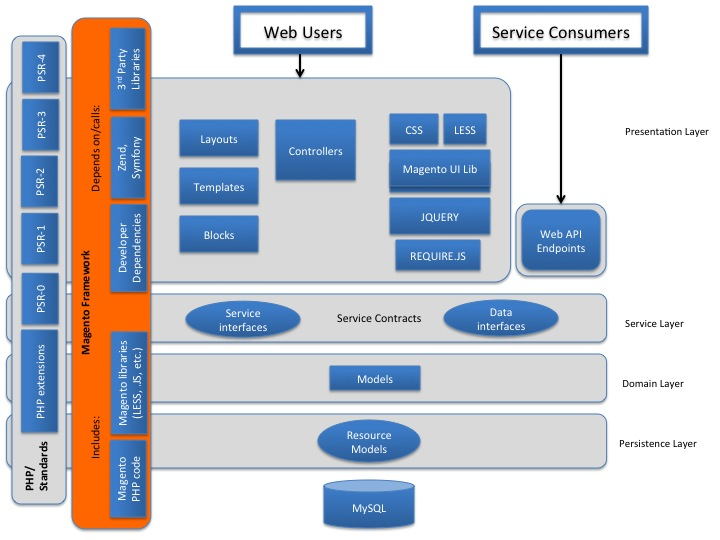
\includegraphics[height=12cm]{images/magento/magento-architecture.jpg}
  \caption{Magento Architecture Overview}
  \label{fig:magento-architecture-overview}
\end{figure}
\vspace{0.5cm}

Interacting with the product and its appearance on a Magento web interface means interacting with presentation layer code composed by both view elements (layouts, blocks, templates) and controllers, which process commands to and from the user interface. 

We can extensively customize this user interface by extending Magento themes capabilities personalizing its content modifying this presentational layer accordingly to the requirements because the theme is responsible for organizing both the visual aspect of the interface and the product behavior.

Each Magento theme resides in a specific directory and includes custom page layouts, templates, skins, and language files that work together to create a distinct user experience.

In our case study example, the Madison Island frontend is built around the technology that we just described using a personalized and customized Magento theme for the user experience on the website. 

\subsection{Layout Updates XML}

Magento offers great flexibility and re-usability of design by layouts defined in XML files. In fact, each Magento module may define its own layout XML file and participate in the process of building the page output. This result is accomplished through a set of instructions contained in these XML files and grouped in \textit{layout handle}s. These directions play a fundamental role to determine the final look and feel of the page returned back to the user.
For example, the handle \textit{catalog\_product\_view} is used to add content to the product detail page, and \textit{checkout\_cart\_index} to the shopping cart page. The following is an excerpt of the \textit{catalog\_category\_default} and  \textit{catalog\_product\_gallery} layout handle instructions contained in the layout XML file liked to the module Magento uses for all the catalog related functionalities (Mage\_Catalog):

\vspace{0.5cm}
\lstset{language=XML}
\begin{lstlisting} 

  <catalog_category_default translate="label">
  <label>Catalog Category (Non-Anchor)</label>
  <reference name="left">
      <block type="catalog/navigation" name="catalog.leftnav" after="currency" template="catalog/navigation/left.phtml"/>
  </reference>
  <reference name="content">
      <block type="catalog/category_view" name="category.products" template="catalog/category/view.phtml">
          <block type="catalog/product_list" name="product_list" template="catalog/product/list.phtml">
              <block type="catalog/product_list_toolbar" name="product_list_toolbar" template="catalog/product/list/toolbar.phtml">
                  <block type="page/html_pager" name="product_list_toolbar_pager"/>
                  <!-- The following code shows how to set your own pager increments -->
                  <!--
                      <action method="setDefaultListPerPage"><limit>4</limit></action>
                      <action method="setDefaultGridPerPage"><limit>9</limit></action>
                      <action method="addPagerLimit"><mode>list</mode><limit>2</limit></action>
                      <action method="addPagerLimit"><mode>list</mode><limit>4</limit></action>
                      <action method="addPagerLimit"><mode>list</mode><limit>6</limit></action>
                      <action method="addPagerLimit"><mode>list</mode><limit>8</limit></action>
                      <action method="addPagerLimit" translate="label"><mode>list</mode><limit>all</limit><label>All</label></action>
                  -->
              </block>
              <action method="addColumnCountLayoutDepend"><layout>empty</layout><count>6</count></action>
              <action method="addColumnCountLayoutDepend"><layout>one_column</layout><count>5</count></action>
              <action method="addColumnCountLayoutDepend"><layout>two_columns_left</layout><count>4</count></action>
              <action method="addColumnCountLayoutDepend"><layout>two_columns_right</layout><count>4</count></action>
              <action method="addColumnCountLayoutDepend"><layout>three_columns</layout><count>3</count></action>
              <action method="setToolbarBlockName"><name>product_list_toolbar</name></action>
          </block>
      </block>
  </reference>
</catalog_category_default>

...

<catalog_product_gallery translate="label">
        <label>Catalog Product Image Gallery Popup</label>
        <!-- Mage_Catalog -->
        <reference name="root">
            <action method="setTemplate"><template>page/popup.phtml</template></action>
        </reference>
        <reference name="content">
            <block type="catalog/product_gallery" name="catalog_product_gallery" template="catalog/product/gallery.phtml"/>
        </reference>
    </catalog_product_gallery>


\end{lstlisting}
\vspace{0.5cm}

As shown above, child nodes are created inside these \textit{layout handle}s to determine which content should appear on any distinct page where these layout handles gets added to an XML structure called \textit{page tree}.

These child nodes are called \textit{block}s, which may, in turn, contain child \textit{block}s of their own. 
Finally, each leaf \textit{block} would contain a template associated to it which would be responsible for displaying some specific content.

\vspace{0.5cm}
\begin{figure}[H]
  \centering
    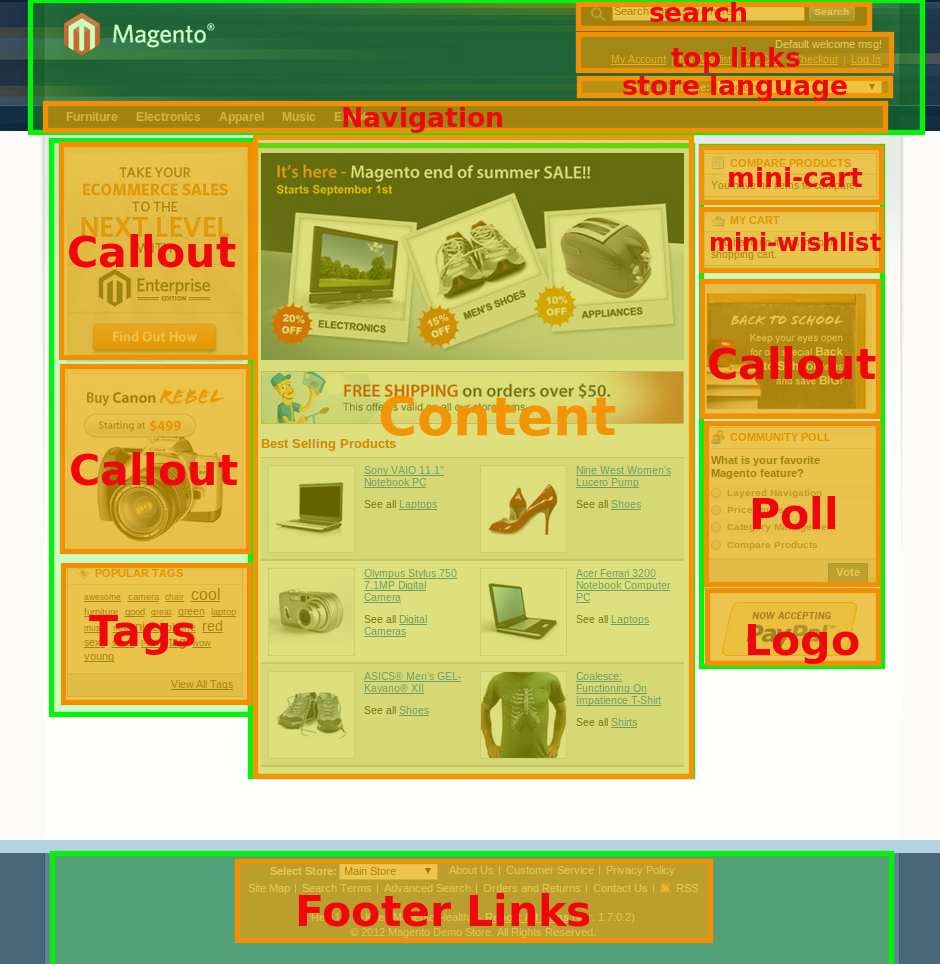
\includegraphics[width=14cm]{images/magento/term-blocks-content.png}
  \caption{Magento content blocks example}
  \label{fig:magento-term-blocks-content}
\end{figure}
\vspace{0.5cm}

In summary, each page of the website can be thought as a composition of Magento \textit{block}s representing a specific page tree configuration. As shown in \ref{fig:magento-madison-island-theme} for the Madison Island theme example, each one of these blocks holds its associated rendering template that gets assembled and internally rendered before being returned to the user browser in the HTTP response.

\vspace{0.5cm}
\begin{figure}[H]
  \centering
    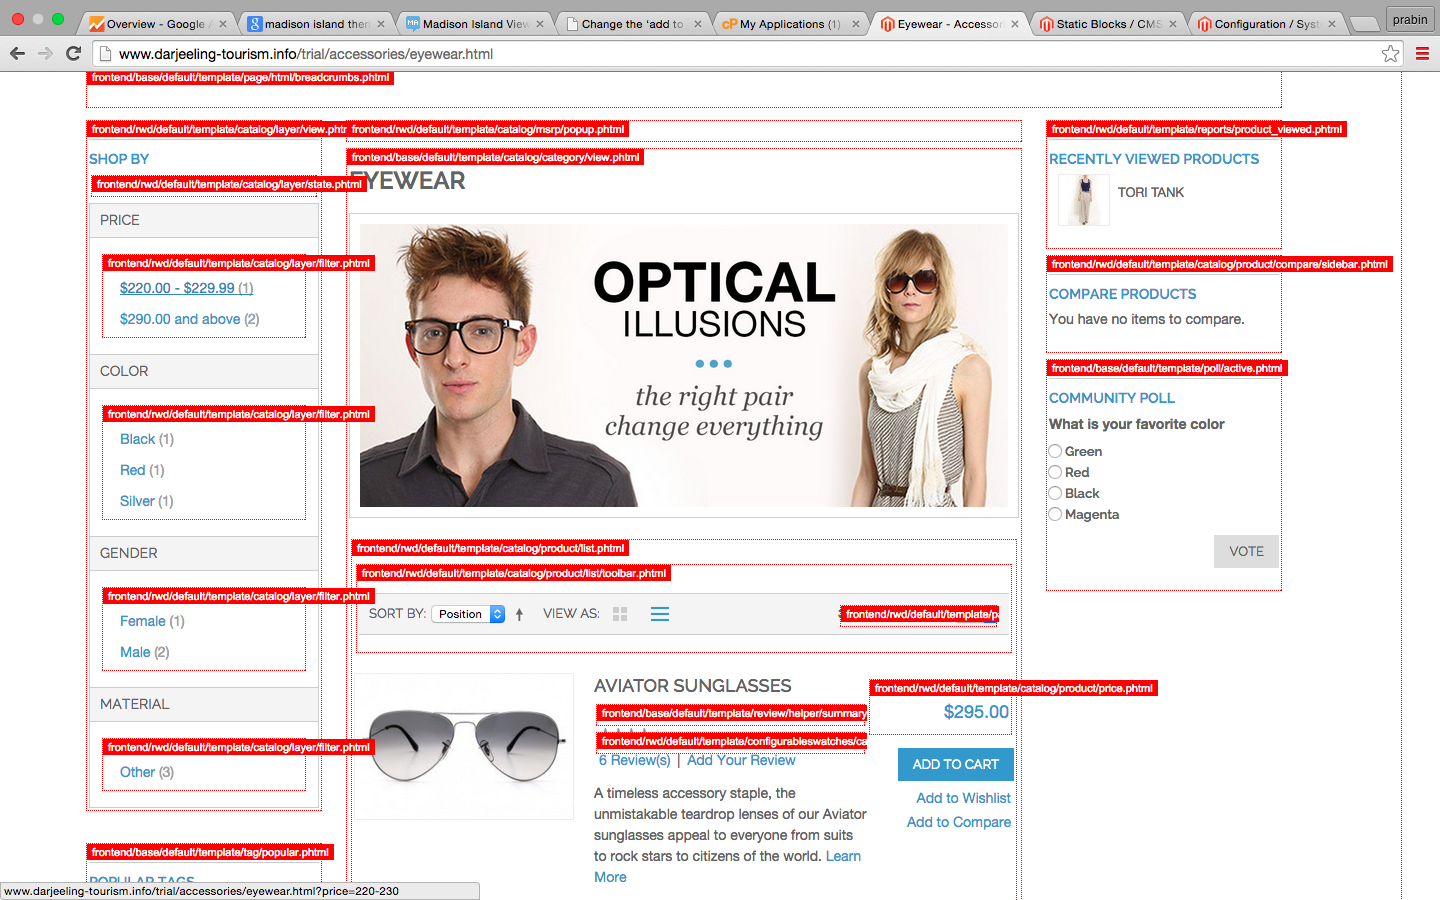
\includegraphics[width=14cm]{images/magento/madison-island-theme.png}
  \caption{Madison Island templates composition}
  \label{fig:magento-madison-island-theme}
\end{figure}
\vspace{0.5cm}

The versatility offered by the Magento rendering engine through the layout update XML mechanism allows us to dynamically append block children under certain conditions or pass parameters to the existing blocks that would affect their rendering behavior. This behavior is beneficial to map the changes we identified through the personalization process integrated within the updated \textit{IFMLModel} describing the enhanced interface offered to the customers on the platform.

In fact, we are in a position now to generate and forward customized XML updates to Magento to reflect those requested changes and efficiently see them implemented on the website.

\newpage
\section{Code generation}

The main idea behind the code generation method is to use the updated \textit{IFMLModel} processed in the previous stage and use it as the input document of an additional transformation capable of generating code understandable by the target platform, in this case, Magento. This generated code would have the form of the Layout Update XML instructions described in the previous section. Finally, these automatically generated XML update snippets will be interpreted and treated from the Magento rendering engine as any other layout update XML file.

\vspace{0.5cm}
\begin{figure}[H]
  \centering
    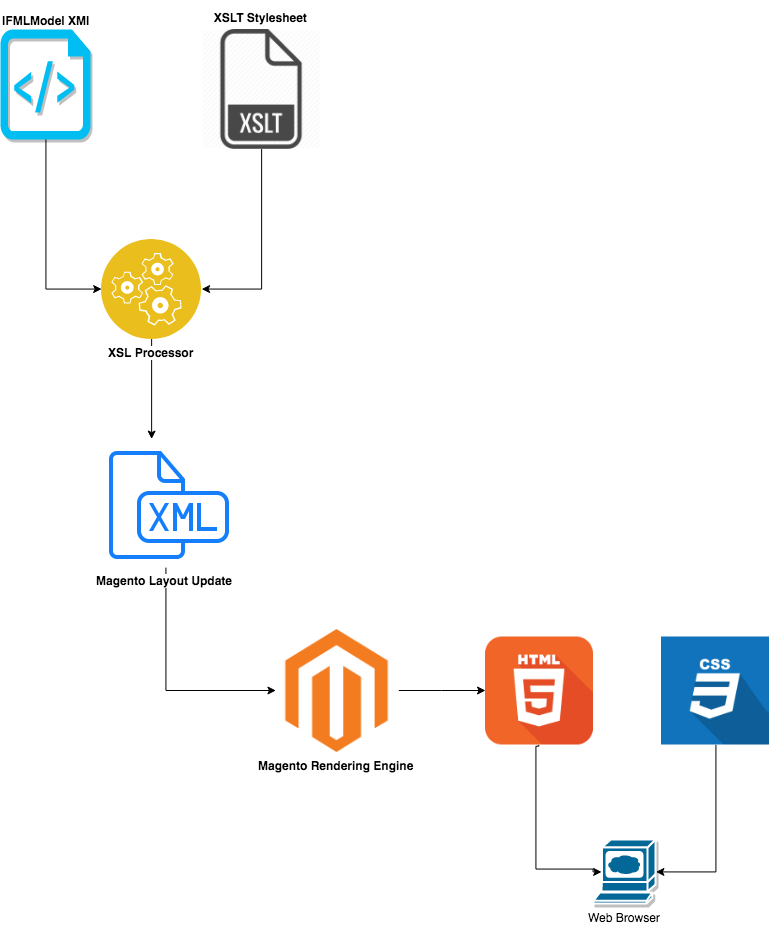
\includegraphics[width=14cm]{images/code-generation.png}
  \caption{Code generation approach}
  \label{fig:code-generation}
\end{figure}
\vspace{0.5cm}

\subsection{XML Metadata Interchange}

XMI (XML Metadata Interchange) is a proposed use of the Extensible Markup Language (XML) that is intended to provide a standard way for programmers and other users to exchange information about metadata (essentially, information about what a set of data consists of and how it is organized)\cite{xmi}. 

Both the \textit{RealDataUsage} and \textit{IFML} models and metamodels definition presented in the previous chapters have been using and persisted throught the XMI specification.

\vspace{0.5cm}
\begin{figure}[H]
  \centering
    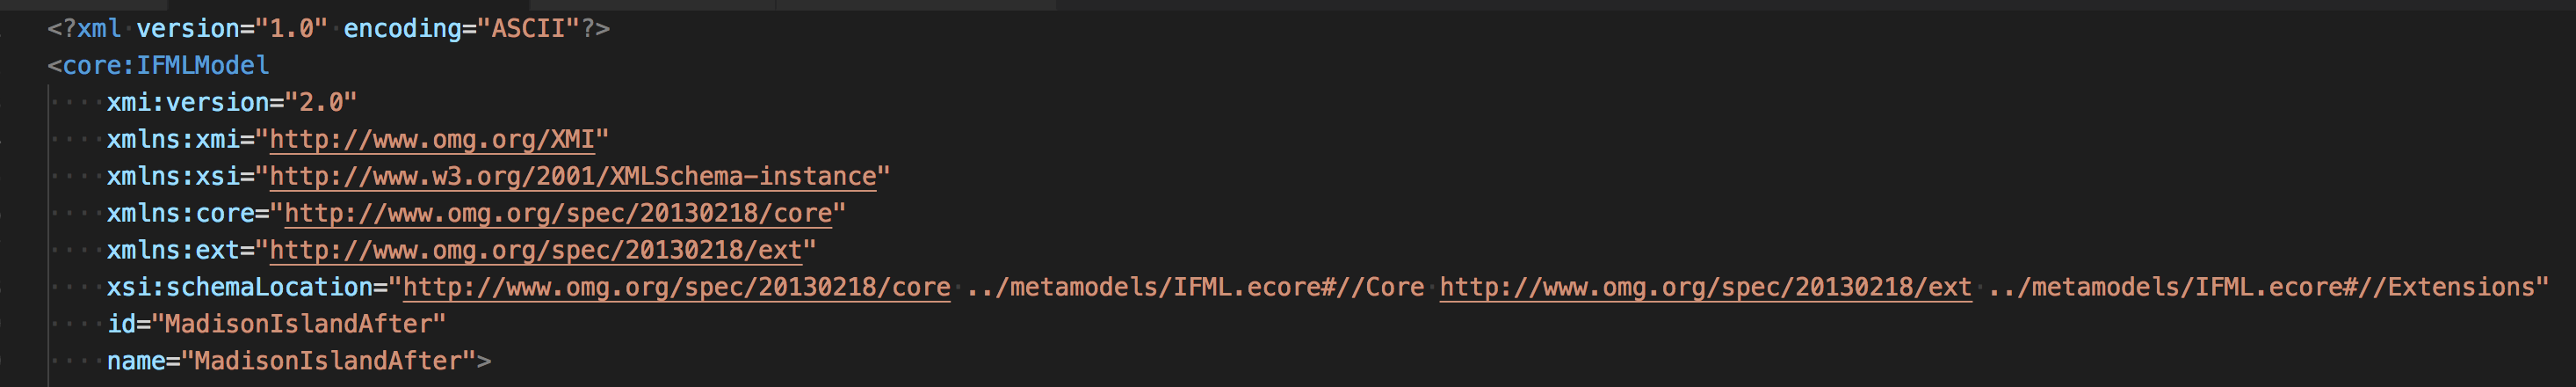
\includegraphics[width=15cm]{images/xmi-header.png}
  \caption{XMI definition for the updated IFMLModel}
  \label{fig:xmi-header}
\end{figure}
\vspace{0.5cm}


Since XMI is XML-based, we decided to employ XSLT to transform the XMI representation of the enhanced \textit{IFMLModel} for code generation of the target documents. 




\subsection{XSL Transformations}

XSL Transformations (XSLT 2.0) is a language for transforming XML documents into other XML documents, text documents or HTML documents\cite{xslt}.

\subsection{Transformation output}


%\addcontentsline{toc}{chapter}{}
